%==============================================================================%
%            PRØVE | FORKURS 1P-2P LÆRERUTDANNING | V2016 | UTSATT             %
%==============================================================================%
%
% __/\\\\\\\\\\\\____________________/\\\\\\___________________/\\\_
%  _\/\\\////////\\\_________________\////\\\_______________/\\\\\\\_
%   _\/\\\______\//\\\___________________\/\\\______________\/////\\\_
%    _\/\\\_______\/\\\_____/\\\\\\\\_____\/\\\__________________\/\\\_
%     _\/\\\_______\/\\\___/\\\/////\\\____\/\\\__________________\/\\\_
%      _\/\\\_______\/\\\__/\\\\\\\\\\\_____\/\\\__________________\/\\\_
%       _\/\\\_______/\\\__\//\\///////______\/\\\__________________\/\\\_
%        _\/\\\\\\\\\\\\/____\//\\\\\\\\\\__/\\\\\\\\\_______________\/\\\_
%         _\////////////_______\//////////__\/////////________________\///_
%
%==============================================================================%
%                              UTEN HJELPEMIDDEL                               %
%==============================================================================%

\Del{u}


%==============================================================================%
%                                 OPPGAVE 1.1                                  %
%==============================================================================%
\Oppgave[3] \points*{3}

Ida målte temperaturen $10$ vinterdager. Resultatet er vist under i
\cref{tab:Forkurs-1p-2p-laererutdanning-2016-V-U-oppgave-1-7}.

\begin{table}[H]
    \centering
    \caption{}
    \label{tab:Forkurs-1p-2p-laererutdanning-2016-V-U-oppgave-1-1}
    \begin{tabular}{|c |S[table-format=1.0]|}
      \tableHeaders{Dato}{Temperatur (\si{\celsius})}
         01.01 &  -7 \\
         02.01 &  -3 \\
         03.01 &   4 \\
         04.01 &   8 \\
         05.01 &  -3 \\
         06.01 & -13 \\
         07.01 &  -3 \\
         08.01 &   8 \\
         09.01 &   0 \\
         10.01 &  -5 \\ \hline
    \end{tabular}
\end{table}

Bestem gjennomsnittet, medianen, typetallet og variasjonsbredden for
temperaturmålingene.


%==============================================================================%
%                                 OPPGAVE 1.2                                  %
%==============================================================================%
\Oppgave[1] \points*{1}

Charlotte blandet saft og vann i forholdet $2:5$. Hun brukte
$\SI{8}{\deci\liter}$. \bigskip

Hvor mange liter ferdig blanding fikk hun?


%==============================================================================%
%                                 OPPGAVE 1.3                                  %
%==============================================================================%
\Oppgave[1] \points*{1}

Prisen for en vare er satt opp med $\SI{20}{\percent}$. Dette tilsvarer en
prisøkning på $120$~kroner. \bigskip

Hvor mye kostet varen før prisen ble satt opp?


%==============================================================================%
%                                 OPPGAVE 1.4                                  %
%==============================================================================%
\Oppgave[1] \points*{1}

Løs likningen
%
\begin{equation*}
  2x - 4 + x = -8 + x - 7
\end{equation*}


%==============================================================================%
%                                 OPPGAVE 1.5                                  %
%==============================================================================%
\Oppgave[2] \points*{2}

Regn ut og skriv svaret på standardform
%
\begin{equation*}
  \frac{\num{72e5}\cdot(\num{e6})^{-3}}{\num{0.06e-4}}
\end{equation*}


%==============================================================================%
%                                 OPPGAVE 1.6                                  %
%==============================================================================%
\Oppgave[3]

\begin{figure}[H]
  \centering
  \tikzsetnextfilename{Forkurs-1p-2p-laererutdanning-2016-V-U-oppgave-1-6}
  \begin{tikzpicture}
    \tkzInit[xmin=-0.4,xmax=9.45,ymin=-0.5,ymax = 7.5]
    \tkzClip

    \def\scale{0.75}
    \pgfmathsetmacro{\AB}{(\scale*12}
    \pgfmathsetmacro{\AC}{(\scale*15}
    \pgfmathsetmacro{\BD}{\scale*7}

    \tkzDefPoint(0,0){A} \tkzDefPoint(\AB,0){B}
    \tkzDefPoint(\AB-\BD,0){D}

    \tkzDefLine[orthogonal=through B](A,B)
    \tkzInterLC[R](B,tkzPointResult)(A,\AC cm) \tkzGetFirstPoint{C}

    \tkzDefLine[orthogonal=through D](A,C)
    \tkzInterLL(A,C)(D,tkzPointResult) \tkzGetPoint{E}

    \tkzMarkRightAngle[thick,color=maincolorMedium,scale=2](D,E,A)
    \tkzMarkRightAngle[thick,color=maincolorMedium,scale=2](A,B,C)
    \tkzDrawSegment[thick,maincolorMedium](D,E)
    \tkzDrawPolygon[thick,maincolorMedium](A,B,C)

    \tkzLabelPoint[below left](A){$A$}
    \tkzLabelPoint[below right](B){$B$}
    \tkzLabelPoint[above right](C){$C$}
    \tkzLabelPoint[below](D){$D$}
    \tkzLabelPoint[above left](E){$E$}
  \end{tikzpicture}
  \caption{}
  \label{fig:Forkurs-1p-2p-laererutdanning-2016-V-U-oppgave-1-6}
\end{figure}

Gitt \cref{fig:Forkurs-1p-2p-laererutdanning-2016-V-U-oppgave-1-6} ovenfor. $AB=12$,
$AC=15$ og $BD=7$.

\begin{oppgaver}
  \Item{1} Forklar hvorfor $\Delta ABC$ og $\Delta AED$ er formlike.
\end{oppgaver}

\begin{oppgaver}
  \Item{2} Bestem arealet av $\Delta AED$ og arealet av $\Delta ABC$.
\end{oppgaver}


%==============================================================================%
%                                 OPPGAVE 1.7                                  %
%==============================================================================%
\Oppgave[1] \points*{1}

\begin{figure}[H]
  \centering
  \tikzsetnextfilename{Forkurs-1p-2p-laererutdanning-2016-V-U-oppgave-1-7}
  \begin{tikzpicture}
    \def\scale{0.75}
    \pgfmathsetmacro{\BC}{(\scale*6}

    \tkzDefPoint(0,0){B} \tkzDefPoint(\BC,0){C}
    \tkzDefSquare(B,C) \tkzGetPoints{D}{E}
    \tkzDefEquilateral(B,E)\tkzGetPoint{A}
    \tkzDefMidPoint(D,C)

    \tkzDrawArc[color=maincolorMedium,thick](tkzPointResult,C)(D)
    \tkzDrawSegments[color=maincolorMedium,thick](B,C E,D B,A A,E)
    \tkzDrawSegments[color=maincolorMedium,dashed,thick](B,E C,D)

    \tkzLabelPoint[left](A){$A$}
    \tkzLabelPoint[below](B){$B$}
    \tkzLabelPoint[below](C){$C$}
    \tkzLabelPoint[above](D){$D$}
    \tkzLabelPoint[above](E){$E$}
  \end{tikzpicture}
  \caption{}
  \label{fig:Forkurs-1p-2p-laererutdanning-2016-V-U-oppgave-1-7}
\end{figure}

En figur er satt sammen av en likesidet trekant, et kvadrat og en halvsirkel.
$C=\SI{6}{\centi\metre}$. Se
\cref{fig:Forkurs-1p-2p-laererutdanning-2016-V-U-oppgave-1-7} ovenfor.
\bigskip

Sett $\pi \approx 3$ og bestem en tilnærmet verdi for omkretsen av figuren.


%==============================================================================%
%                                 OPPGAVE 1.8                                  %
%==============================================================================%
\Oppgave[2] \points*{2}

I en gruppe er det $2$~gutter og  $5$~jenter. Lærerene skal trekke $2$ elever
tilfeldig fra gruppen. \bigskip

Bestem sannsynligheten for at læreren kommer til å trekke ut én gutt og én
jente.


%==============================================================================%
%                                 OPPGAVE 1.9                                  %
%==============================================================================%
\Oppgave[4]

\begin{figure}[H]
  \centering
  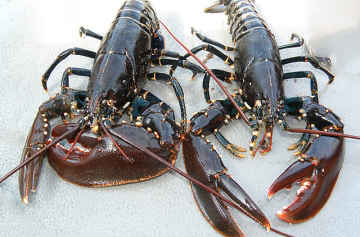
\includegraphics[width=0.6\textwidth]{Forkurs-1p-2p-laererutdanning-2016-V-U-oppgave-1-9-hummer.jpg}
\end{figure}

Eivind fisker hummere. Han har skrevet ned hvor mange hummere han fikk hver dag
de $18$ dagene i hummerfisket. Se \cref{tab:Forkurs-2016-H-oppgave-1.9a}.

\begin{table}[H]
  \centering
  \caption{}
  \label{tab:Forkurs-1p-2p-laererutdanning-2016-V-U-oppgave-1-9a}
  \begin{tabularx}{\textwidth}{| l | *{9}{Z|} }
    \hline
    \Cellcolor Dag            &  1 &  2 &  3 &  4 &  5 &  6 &  7 &  8 &  9  \\
    \hline
    \Cellcolor Antall hummere & 23 & 18 & 24 & 15 & 29 & 16 & 26 & 20 & 12 \\
    \hline
  \end{tabularx} \bigskip

  \begin{tabularx}{\textwidth}{| l | *{9}{Z|} }
    \hline
    \Cellcolor Dag            & 10 & 11 & 12 & 13 & 14 & 15 & 16 & 17 & 18 \\
    \hline
    \Cellcolor Antall hummere & 10 &  7 & 12 &  9 & 17 &  4 &  8 &  9 & 13 \\
    \hline
  \end{tabularx}
\end{table}

\begin{oppgaver}
  \Item{2} Tegn av og fyll ut
  \cref{tab:Forkurs-1p-2p-laererutdanning-2016-V-U-oppgave-1-9a}. Bestem
    gjenomsnittet for det klassedelte datamaterialet.
\end{oppgaver}

\begin{table}[H]
  \centering
  \caption{}
  \label{tab:Forkurs-1p-2p-laererutdanning-2016-V-U-oppgave-1-9b}
  \begin{tabular}{|c | c|}
    \tableHeaders{Lengde ($\si{\km}$)}{Antall uker}
    $\left[\phantom{1}0, 10\right\rangle$ & \\
    $\left[          10, 15\right\rangle$ & \\
    $\left[          15, 20\right\rangle$ & \\
    $\left[          20, 30\right\rangle$ & \\
    \hline
  \end{tabular}
\end{table}

\begin{oppgaver}
  \Item{2} Lag et histogram som viser fordelingen i
    \cref{tab:Forkurs-1p-2p-laererutdanning-2016-V-U-1-7b}.
\end{oppgaver}


%==============================================================================%
%                                 OPPGAVE 1.10                                 %
%==============================================================================%
\Oppgave[2] \points*{2}

\begin{table}[H]
  \centering
  \label{tab:Forkurs-1p-2p-laererutdanning-2016-V-U-oppgave-1-10}
  \begin{tabular}{| S[table-format=4.0] | S[table-format=3.1] |}
    \tableHeaders{År}{Pris for en kroneis}
      1972 &  20.4 \\
      2015 & 139.8 \\ \hline
  \end{tabular}
\end{table}

I $1972$ hadde Ådne en nominell lønn på $\num{40000}$~kroner. I $2015$ hadde
Ådnes datter en nominell lønn på $\num{420000}$~kroner. \bigskip

Hvem av de to hadde størst kjøpekraft?


%==============================================================================%
%                                 OPPGAVE 1.11                                 %
%==============================================================================%
\Oppgave[2] \points*{2}

Gi et eksempel på en sammenheng fra virkeligheten som kan beskrives med en
lineær funksjon. Bestem funksjonsuttrykket og lag en skisse av grafen til
funksjonen.


%==============================================================================%
%                                 OPPGAVE 1.12                                 %
%==============================================================================%
\Oppgave[2] \points*{2}

Tenk deg at du oppretter en konto i banken og setter inn $\num{8000}$~kroner. Du
får en fast prosent rente per år. Ett år etter at du satte inn pengene, har du
$\num{8200}$~kroner kroner på kontoen. \bigskip

Bestem et funksjonsutrykk $f(x)$ som viser hvor mye du vil ha på kontoen $x$ år
etter at du satte inn pengene.



